\documentclass[t,12pt]{beamer}
\usepackage[utf8]{inputenc}
\usepackage[T1]{fontenc}
\usepackage{fancyhdr} % pour personnaliser les en-têtes
\usepackage{lastpage}
\usepackage[frenchb]{babel}
\usepackage{amsfonts,amssymb}
\usepackage{amsmath,amsthm}
\usepackage{paralist}
\usepackage{enumerate}
\usepackage{xspace}
\usepackage{xcolor}
\usepackage{variations}
\usepackage{xypic}
\usepackage{eurosym,multicol}
\usepackage{graphicx}
\usepackage[np]{numprint}
\usepackage{hyperref} 
\usepackage{setspace}
\usepackage{listings} % pour écrire des codes avec coloration syntaxique  

\usepackage{tikz}
\usetikzlibrary{calc, arrows, plotmarks,decorations.pathreplacing}
\usepackage{colortbl}
\usepackage{multirow}


\newtheorem{defi}{Définition}
\newtheorem{thm}{Théorème}
\newtheorem{thm-def}{Théorème/Définition}
\newtheorem{rmq}{Remarque}
\newtheorem{prop}{Propriété}
\newtheorem{cor}{Corollaire}
\newtheorem{lem}{Lemme}
\newtheorem{ex}{Exemple}
\newtheorem{cex}{Contre-exemple}
\newtheorem{prop-def}{Propriété-définition}
\newtheorem{exer}{Exercice}
\newtheorem{nota}{Notation}
\newtheorem{ax}{Axiome}
\newtheorem{appl}{Application}
\newtheorem{csq}{Conséquence}
%\def\di{\displaystyle}


\newcommand{\vtab}{\rule[-0.4em]{0pt}{1.2em}}
\newcommand{\V}{\overrightarrow}
\renewcommand{\thesection}{\Roman{section} }
\renewcommand{\thesubsection}{\arabic{subsection} }
\renewcommand{\thesubsubsection}{\alph{subsubsection} }
\newcommand{\C}{\mathbb{C}}
\newcommand{\R}{\mathbb{R}}
\newcommand{\Q}{\mathbb{Q}}
\newcommand{\Z}{\mathbb{Z}}
\newcommand{\N}{\mathbb{N}}


\definecolor{vert}{RGB}{11,160,78}
\definecolor{rouge}{RGB}{255,120,120}


\usetheme{Warsaw}

\title{Questions sur la lecture graphique}
%\author{Évaluation de 30 minutes \\jeudi 17 mars 2022}
\date{}
\begin{document}
\maketitle	

\begin{frame}
	\frametitle{Question 1: }
$$\shorthandoff{:}\begin{tikzpicture}[xscale=1, yscale = 0.8]
\clip (-3.5,-3.5) rectangle (3.5,3.5);
\draw[step=0.5,dotted] (-3.5,-3.5) grid (3.5,3.5);
\draw [->, line width = 1pt, >=latex'](-3.5,0) -- (3.5,0);
\draw (3.4,0) node[below]{\footnotesize$x$};
\draw (0,3.2) node[right]{\footnotesize$y$};
\foreach \x in {-3,-2,-1,1,2,3}
\draw[shift={(\x,0)}] (0pt,2pt) -- (0pt,-2pt) node[below] {\tiny $\x$};
\draw [->, line width = 1pt, >=latex'](0,-3.5) -- (0,3.5);
\foreach \y in {-3,-2,-1,1,2,3}
\draw[shift={(0,\y)}] (2pt,0pt) -- (-2pt,0pt) node[left] {\tiny $\y$};
\draw (0,0) node[below right]{\tiny $0$};
\draw[domain=-3.5:3.5,samples=200,color=blue] plot ({\x},{2.5*sin(pi*\x r)});
\draw (2.6,2.7) node[left]{\footnotesize$\mathcal{C}_h$};
\end{tikzpicture}\shorthandon{:}$$
	\hfill\\[-0.2cm]\begin{enumerate}
		\item Donner deux antécédents de $2.5$ par la fonction $h$.
		\item Donner l'image de  de $0.5$ par la fonction $h$.
		%\item Combien d'antécédents de zéro possède la fonction $h$ sur ce graphique? 
	\end{enumerate}

\end{frame}

\begin{frame}
	\frametitle{Question 2:  }
	
$$\shorthandoff{:}\begin{tikzpicture}[xscale=0.9, yscale = 0.7]
\clip (-3.5,-3.5) rectangle (3.5,3.5);
\draw[step=0.5,dotted] (-3.5,-3.5) grid (3.5,3.5);
\draw [->, line width = 1pt, >=latex'](-3.5,0) -- (3.5,0);
\draw (3.4,0) node[below]{\footnotesize$x$};
\draw (0,3.2) node[right]{\footnotesize$y$};
\foreach \x in {-3,-2,-1,1,2,3}
\draw[shift={(\x,0)}] (0pt,2pt) -- (0pt,-2pt) node[below] {\tiny $\x$};
\draw [->, line width = 1pt, >=latex'](0,-3.5) -- (0,3.5);
\foreach \y in {-3,-2,-1,1,2,3}
\draw[shift={(0,\y)}] (2pt,0pt) -- (-2pt,0pt) node[left] {\tiny $\y$};
\draw (0,0) node[below right]{\tiny $0$};
\draw[domain=-3.5:3.5,samples=100,color=blue] plot ({\x},{2.5*cos(pi*\x/2 r)});
\draw (1.6,3) node[left]{\footnotesize$\mathcal{C}_g$};
\end{tikzpicture}\shorthandon{:}$$
\hfill\\[-0.2cm]\begin{enumerate}
	\item Combien d'antécédents de zéro possède la fonction $g$ sur ce graphique?
	\item Que pouvez-vous dire sur la parité de la fonction $g$?  
\end{enumerate}

\end{frame}

\begin{frame}
	\frametitle{Question 3: }



\begin{figure}[t]
	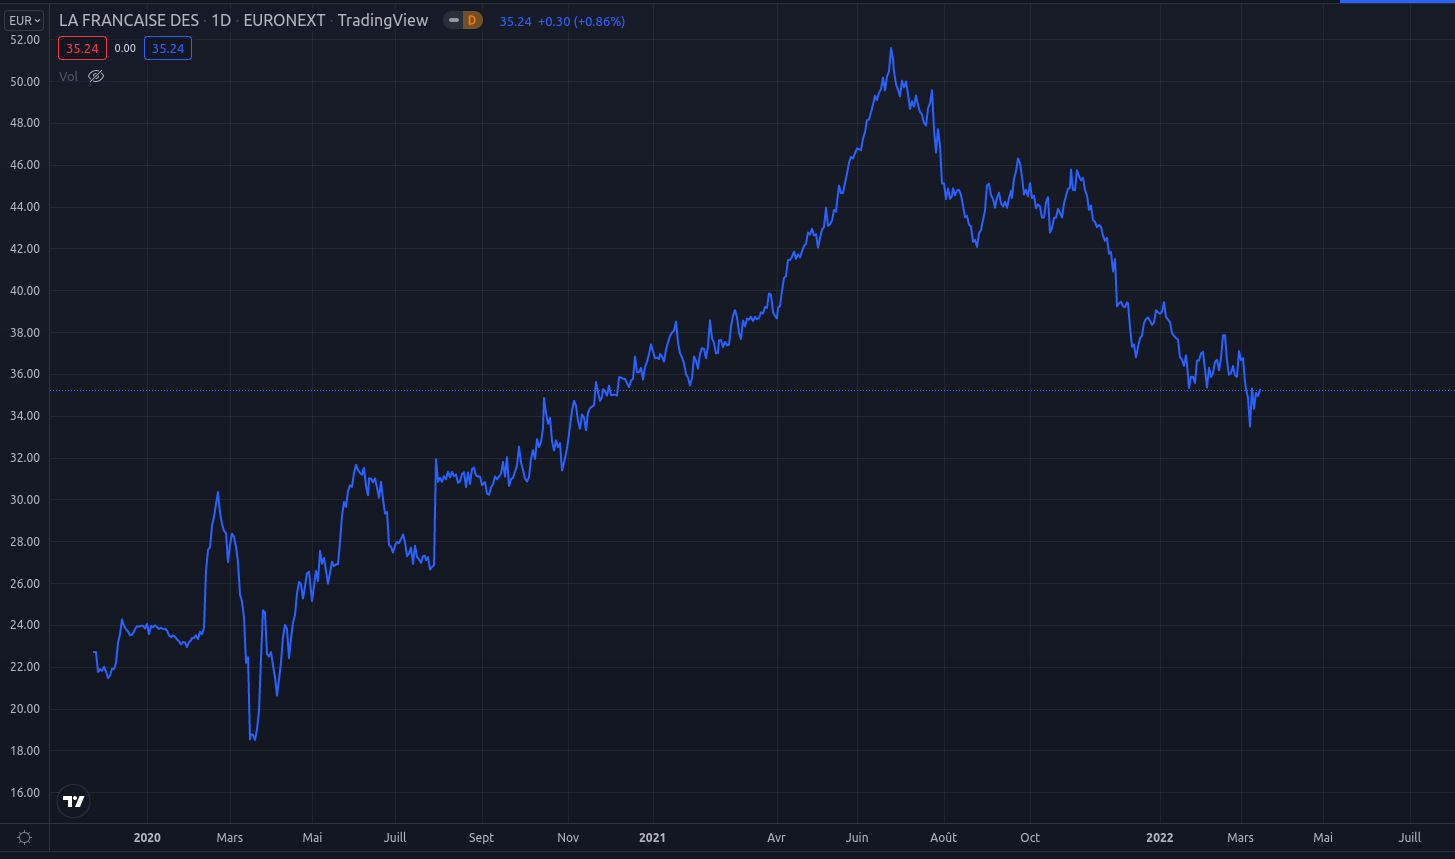
\includegraphics[width=8.5cm]{fdj.png}
	\centering
\end{figure}

\noindent Voici ci-dessus la courbe représentative du prix de l'action FDJ en fonction du temps depuis son introduction en bourse le 21 novembre 2019.\\ Donner l'image la plus haute et l'image la plus basse associées respectivement à la courbe ci-dessus. 

	

\end{frame}

\begin{frame}
	\frametitle{Question 4:}
	
$$\shorthandoff{:}\begin{tikzpicture}[xscale=0.9, yscale = 0.7]
\clip (-3.5,-3.5) rectangle (3.5,3.5);
\draw[step=0.5,dotted] (-3.5,-3.5) grid (3.5,3.5);
\draw [->, line width = 1pt, >=latex'](-3.5,0) -- (3.5,0);
\draw (3.4,0) node[below]{\footnotesize$x$};
\draw (0,3.2) node[right]{\footnotesize$y$};
\foreach \x in {-3,-2,-1,1,2,3}
\draw[shift={(\x,0)}] (0pt,2pt) -- (0pt,-2pt) node[below] {\tiny $\x$};
\draw [->, line width = 1pt, >=latex'](0,-3.5) -- (0,3.5);
\foreach \y in {-3,-2,-1,1,2,3}
\draw[shift={(0,\y)}] (2pt,0pt) -- (-2pt,0pt) node[left] {\tiny $\y$};
\draw (0,0) node[below right]{\tiny $0$};
\draw[domain=-3.5:3.5,samples=100,color=blue] plot ({\x},{0.4*(\x+2.5)*(\x-3)});
\draw (3.4,1.5) node[left]{\footnotesize$\mathcal{C}_H$};
\end{tikzpicture}\shorthandon{:}$$
\hfill\\[-0.2cm]\begin{enumerate}
	\item Donner le tableau de signes de la fonction $H$. 
	\item Donner le tableau de variations de la fonction $H$.  
\end{enumerate}
	
 

\end{frame}

\begin{frame}
	\frametitle{Question 5: }

$$\shorthandoff{:}\begin{tikzpicture}[xscale=0.9, yscale = 0.7]
\clip (-3.5,-3.5) rectangle (3.5,3.5);
\draw[step=0.5,dotted] (-3.5,-3.5) grid (3.5,3.5);
\draw [->, line width = 1pt, >=latex'](-3.5,0) -- (3.5,0);
\draw (3.4,0) node[below]{\footnotesize$x$};
\draw (0,3.2) node[right]{\footnotesize$y$};
\foreach \x in {-3,-2,-1,1,2,3}
\draw[shift={(\x,0)}] (0pt,2pt) -- (0pt,-2pt) node[below] {\tiny $\x$};
\draw [->, line width = 1pt, >=latex'](0,-3.5) -- (0,3.5);
\foreach \y in {-3,-2,-1,1,2,3}
\draw[shift={(0,\y)}] (2pt,0pt) -- (-2pt,0pt) node[left] {\tiny $\y$};
\draw (0,0) node[below right]{\tiny $0$};
\draw[domain=-3.5:3.5,samples=100,color=blue] plot ({\x},{0.2*(\x+2.5)*(\x-3)*(\x+0.5)});
\draw (3.4,1.5) node[left]{\footnotesize$\mathcal{C}_V$};
\end{tikzpicture}\shorthandon{:}$$
\hfill\\[-0.2cm]\begin{enumerate}
	\item Donner le tableau de signes de la fonction $V$. 
	\item Donner le tableau de variations de la fonction $V$.  
\end{enumerate}
	
\end{frame}


\begin{frame}
	\frametitle{Question 6}
$$\shorthandoff{:}\begin{tikzpicture}[xscale=0.9, yscale = 0.7]
\clip (-3.5,-2.5) rectangle (3.5,3.5);
\draw[step=0.5,dotted] (-3.5,-2.5) grid (3.5,3.5);
\draw [->, line width = 1pt, >=latex'](-3.5,0) -- (3.5,0);
\draw (3.4,0) node[below]{\footnotesize$x$};
\draw (0,3.2) node[right]{\footnotesize$y$};
\foreach \x in {-3,-2,-1,1,2,3}
\draw[shift={(\x,0)}] (0pt,2pt) -- (0pt,-2pt) node[below] {\tiny $\x$};
\draw [->, line width = 1pt, >=latex'](0,-3.5) -- (0,3.5);
\foreach \y in {-2,-1,1,2,3}
\draw[shift={(0,\y)}] (2pt,0pt) -- (-2pt,0pt) node[left] {\tiny $\y$};
\draw (0,0) node[below right]{\tiny $0$};
\draw[domain=-3.5:3.5,samples=100,color=blue] plot ({\x},{0.75*\x+0.5});
\draw[domain=-3.5:3.5,samples=100,color=red] plot ({\x},{-0.5*\x+0.5});
\draw[domain=-3.5:3.5,samples=100,color=olive] plot ({\x},{1.5});
\draw (3.3,1.8) node[left]{\footnotesize$\mathcal{C}_f$};
\draw (3.3,3.2) node[left]{\footnotesize$\mathcal{C}_g$};
\draw (3.3,-1.4) node[left]{\footnotesize$\mathcal{C}_h$};
\end{tikzpicture}\shorthandon{:}$$
\hfill\\[-0.2cm]\begin{enumerate}
	\item Résoudre graphiquement $f(x)=h(x)$. 
	\item Résoudre graphiquement $h(x)\leq g(x)$.
	\item Résoudre graphiquement $f(x)\geq g(x)$.   
\end{enumerate}
\end{frame}







\end{document}